\documentclass[10pt,a4paper,landscape]{article}

\usepackage[margin=1.15cm]{geometry}
\usepackage{amsmath,amssymb}
\usepackage[version=4]{mhchem}
\usepackage{amsmath,amssymb,mathtools}
\usepackage{chemfig}
\usepackage{tikz}
\usepackage{xcolor}
\usepackage{booktabs}
\usepackage{hyperref}
\usepackage{pdflscape}
\usepackage{microtype}

\usetikzlibrary{arrows.meta,positioning,calc}

\setlength{\parindent}{0pt}
\setlength{\parskip}{4pt}
\setlength{\tabcolsep}{5pt}
\renewcommand{\arraystretch}{1.25}

\setchemfig{
  atom sep=1.7em,
  bond style={line width=0.8pt},
  double bond sep=2pt
}

\definecolor{phos}{RGB}{30,90,190}
\definecolor{redox}{RGB}{185,55,45}
\definecolor{enz}{RGB}{20,115,75}
\definecolor{carbon}{RGB}{45,45,45}
\definecolor{lightbg}{RGB}{245,247,250}

\hypersetup{
  colorlinks=true,
  linkcolor=blue!60!black
}

% =========================================================
% STRUCTURAL FORMULAS
% Open-chain structures. Stereochemistry is omitted.
% =========================================================

% Glucose: C1 aldehyde; C6 primary alcohol
\newcommand{\Glucose}{%
  \chemfig{
    H-C(=[2]O)-C(-[2]OH)(-[6]H)
    -C(-[2]OH)(-[6]H)
    -C(-[2]OH)(-[6]H)
    -C(-[2]OH)(-[6]H)
    -CH_2OH
  }%
}

% Glucose-6-phosphate
\newcommand{\GsixP}{%
  \chemfig{
    H-C(=[2]O)-C(-[2]OH)(-[6]H)
    -C(-[2]OH)(-[6]H)
    -C(-[2]OH)(-[6]H)
    -C(-[2]OH)(-[6]H)
    -CH_2-O-P(=[2]O)(-[6]OH)-OH
  }%
}

% Fructose-6-phosphate: C2 ketone
\newcommand{\FsixP}{%
  \chemfig{
    CH_2OH-C(=[2]O)-C(-[2]OH)(-[6]H)
    -C(-[2]OH)(-[6]H)
    -C(-[2]OH)(-[6]H)
    -CH_2-O-P(=[2]O)(-[6]OH)-OH
  }%
}

% Fructose-1,6-bisphosphate
\newcommand{\FbisP}{%
  \chemfig{
    CH_2-O-P(=[2]O)(-[6]OH)-OH
    -[0]C(=[2]O)
  }%
}

% DHAP: ketone at C2; phosphate at C3
\newcommand{\DHAP}{%
  \chemfig{
    HO-CH_2-C(=[2]O)-CH_2-O-P(=[2]O)(-[6]OH)-OH
  }%
}

% GAP: aldehyde at C1; phosphate at C3
\newcommand{\GAP}{%
  \chemfig{
    H-C(=[2]O)-C(-[2]OH)(-[6]H)
    -CH_2-O-P(=[2]O)(-[6]OH)-OH
  }%
}

% 1,3-bisphosphoglycerate:
% C1 acyl phosphate; C3 phosphate ester
\newcommand{\BPG}{%
  \chemfig{
    O=C(-[6]O-P(=[2]O)(-[6]OH)-OH)
    -C(-[2]OH)(-[6]H)
    -CH_2-O-P(=[2]O)(-[6]OH)-OH
  }%
}

% 3-phosphoglycerate
\newcommand{\PGthree}{%
  \chemfig{
    HO-C(=[2]O)-C(-[2]OH)(-[6]H)
    -CH_2-O-P(=[2]O)(-[6]OH)-OH
  }%
}

% 2-phosphoglycerate
\newcommand{\PGtwo}{%
  \chemfig{
    HO-C(=[2]O)-C(-[2]O-P(=[2]O)(-[6]OH)-OH)(-[6]H)
    -CH_2OH
  }%
}

% Phosphoenolpyruvate
\newcommand{\PEP}{%
  \chemfig{
    HO-C(=[2]O)-C(-[2]O-P(=[2]O)(-[6]OH)-OH)=CH_2
  }%
}

% Pyruvate
\newcommand{\Pyruvate}{%
  \chemfig{
    HO-C(=[2]O)-C(=[2]O)-CH_3
  }%
}

% =========================================================
% DOCUMENT
% =========================================================

\begin{document}

\begin{center}
{\LARGE\bfseries Glycolysis: Complete Molecular Reaction Map}

\vspace{2mm}

{\large Ten enzyme-catalysed reactions, molecular structures,
phosphate transfers, and redox accounting}

\vspace{2mm}

\textbf{Pathway:}
Glucose $\rightarrow$ 2 Pyruvate

\textbf{Net yield per glucose:}
2 ATP, 2 NADH, 2 pyruvate
\end{center}

\hrule
\vspace{3mm}

\section*{Structural notation}

\begin{itemize}
  \item \textcolor{phos}{Blue}: phosphate transfer or phosphate-bearing group.
  \item \textcolor{redox}{Red}: oxidation-reduction bookkeeping.
  \item \textcolor{enz}{Green}: enzyme label.
  \item Carbon skeletons are shown in open-chain form.
  \item Protonation states are schematic; physiological forms depend
  on pH and the ionic environment.
\end{itemize}

\textbf{Important:} The displayed structural formulas are intended
to show connectivity and functional-group changes. They omit
stereochemistry and do not represent every enzyme-bound intermediate.

% =========================================================
\section*{PHASE I: ENERGY INVESTMENT}
% =========================================================

\subsection*{STEP 1. Glucose $\rightarrow$ Glucose-6-phosphate}

\textcolor{enz}{\textbf{Enzyme: Hexokinase}}

\[
\ce{Glucose + ATP -> Glucose-6-phosphate + ADP}
\]

\begin{center}
\resizebox{0.94\linewidth}{!}{$
\begin{aligned}
\text{\textbf{Glucose:}}\quad
&\Glucose
\\[5pt]
&\xrightarrow[\text{Mg}^{2+}]
{\text{Hexokinase;\ ATP}\rightarrow\text{ADP}}
\\[5pt]
\text{\textbf{Glucose-6-phosphate:}}\quad
&\GsixP
\end{aligned}
$}
\end{center}

\textbf{Chemical changes}

\begin{enumerate}
  \item The oxygen of the C6 hydroxyl group participates in
  phosphoryl transfer.
  \item The terminal phosphoryl group of ATP is transferred
  to the C6 oxygen.
  \item The C6 group changes from $\ce{-CH2OH}$ to
  $\ce{-CH2OPO3H2}$ in the schematic formula.
  \item ATP becomes ADP.
\end{enumerate}

\textcolor{phos}{\textbf{Transfer:}}
\[
\ce{ATP -> ADP + phosphate\ transferred\ to\ glucose}
\]

\textbf{Redox:} No net oxidation or reduction occurs.

\textbf{Atom accounting:} All six glucose carbon atoms are retained.

\[
\boxed{\text{ATP consumed: 1}}
\]

% =========================================================

\subsection*{STEP 2. Glucose-6-phosphate $\rightarrow$ Fructose-6-phosphate}

\textcolor{enz}{\textbf{Enzyme: Phosphoglucose isomerase}}

\[
\ce{Glucose-6-phosphate <=> Fructose-6-phosphate}
\]

\begin{center}
\resizebox{0.94\linewidth}{!}{$
\begin{aligned}
&\GsixP
\\[5pt]
&\xrightleftharpoons{\text{Phosphoglucose isomerase}}
\\[5pt]
&\FsixP
\end{aligned}
$}
\end{center}

\textbf{Chemical changes}

\begin{enumerate}
  \item The cyclic sugar can open into its linear form.
  \item The aldehyde functionality at C1 is converted into a
  ketone functionality at C2.
  \item The reaction proceeds through an enediol or
  enediolate-like intermediate.
  \item Proton transfer and carbonyl reformation yield
  fructose-6-phosphate.
\end{enumerate}

\textbf{Electron movement:} Bond electrons are redistributed
within the sugar. There is no net electron transfer to NAD$^+$.

\textbf{Phosphate accounting:} The phosphate remains attached at C6.

\[
\boxed{\text{ATP consumed: 0}}
\]

% =========================================================

\subsection*{STEP 3. Fructose-6-phosphate $\rightarrow$ Fructose-1,6-bisphosphate}

\textcolor{enz}{\textbf{Enzyme: Phosphofructokinase-1 (PFK-1)}}

\[
\ce{
Fructose-6-phosphate + ATP
-> Fructose-1,6-bisphosphate + ADP
}
\]

\begin{center}
\[
\boxed{
\ce{F6P + ATP ->[PFK-1][Mg^{2+}] F1,6BP + ADP}
}
\]
\end{center}

\textbf{Chemical changes}

\begin{enumerate}
  \item The C1 hydroxyl group is phosphorylated.
  \item ATP donates a terminal phosphoryl group.
  \item The pre-existing phosphate at C6 is retained.
  \item The product now has phosphate groups at C1 and C6.
\end{enumerate}

\textcolor{phos}{\textbf{Transfer:}}
\[
\ce{ATP -> ADP}
\]

A phosphate group is added to the C1 oxygen of the sugar.

\textbf{Redox:} No net oxidation-reduction reaction occurs.

\[
\boxed{\text{ATP consumed: 1}}
\]

\[
\boxed{\text{Cumulative ATP investment: 2}}
\]

% =========================================================

\subsection*{STEP 4. Fructose-1,6-bisphosphate cleavage}

\textcolor{enz}{\textbf{Enzyme: Aldolase}}

\[
\ce{
Fructose-1,6-bisphosphate
<=> GAP + DHAP
}
\]

\begin{center}
\begin{tikzpicture}[
  mol/.style={align=center},
  rx/.style={-{Stealth[length=3mm]},thick},
  node distance=9mm
]
\node[mol] (substrate) {
  \textbf{Six-carbon substrate}\\[2mm]
  \fbox{Fructose-1,6-bisphosphate}\\
  \small C$_6$; phosphates at C1 and C6
};

\node[mol,below=of substrate] (enzyme) {
  \textcolor{enz}{\textbf{Aldolase}}\\
  \small Cleaves the C3--C4 bond
};

\node[mol,below left=12mm and 25mm of enzyme] (gap) {
  \textbf{Glyceraldehyde-3-phosphate}\\[2mm]
  \GAP\\
  \small C$_3$; aldehyde
};

\node[mol,below right=12mm and 25mm of enzyme] (dhap) {
  \textbf{Dihydroxyacetone phosphate}\\[2mm]
  \DHAP\\
  \small C$_3$; ketone
};

\draw[rx] (substrate) -- (enzyme);
\draw[rx] (enzyme) -- (gap);
\draw[rx] (enzyme) -- (dhap);
\end{tikzpicture}
\end{center}

\textbf{Chemical changes}

\begin{enumerate}
  \item The six-carbon substrate undergoes carbon-carbon bond cleavage.
  \item The bond between C3 and C4 is broken.
  \item One three-carbon product is GAP.
  \item The other three-carbon product is DHAP.
  \item Both products contain a phosphate group.
\end{enumerate}

\textbf{Electron movement:} Bond electrons are redistributed during
the cleavage mechanism. The net reaction is not an oxidation-reduction
reaction.

\[
\boxed{\mathrm{C_6 \longrightarrow C_3+C_3}}
\]

No carbon dioxide is released.

% =========================================================

\subsection*{STEP 5. DHAP $\rightleftharpoons$ GAP}

\textcolor{enz}{\textbf{Enzyme: Triose phosphate isomerase}}

\[
\ce{
Dihydroxyacetone phosphate
<=> Glyceraldehyde-3-phosphate
}
\]

\begin{center}
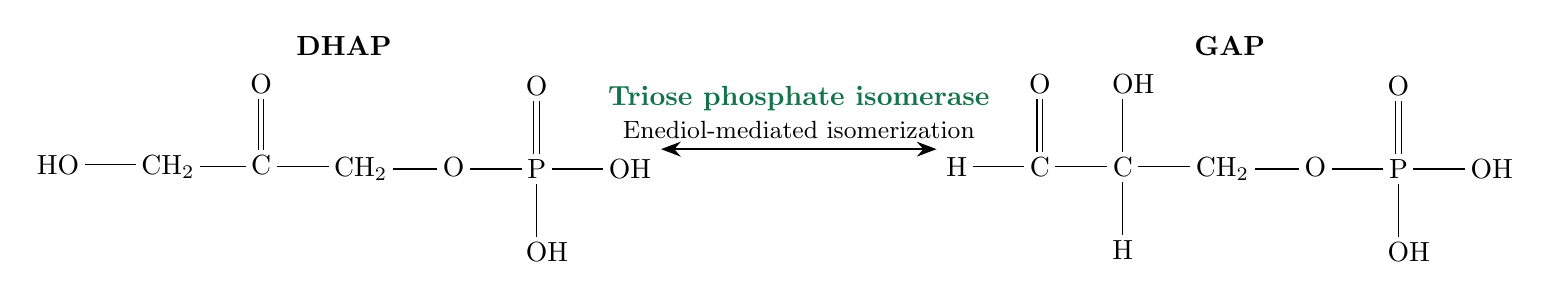
\begin{tikzpicture}[
  mol/.style={align=center},
  rx/.style={{Stealth[length=2.5mm]}-{Stealth[length=2.5mm]},thick},
  node distance=15mm
]

\node[mol] (dhap) {
  \textbf{DHAP}\\[2mm]
  \DHAP
};

\node[mol,right=35mm of dhap] (gap) {
  \textbf{GAP}\\[2mm]
  \GAP
};

\draw[rx] (dhap) -- node[above,align=center] {
  \textcolor{enz}{\textbf{Triose phosphate isomerase}}\\
  \small Enediol-mediated isomerization
} (gap);

\end{tikzpicture}
\end{center}

\textbf{Chemical changes}

\begin{enumerate}
  \item The ketone functionality of DHAP is converted into
  the aldehyde functionality of GAP.
  \item A proton is transferred through the enzyme-catalysed
  mechanism.
  \item The three-carbon skeleton and phosphate group are retained.
\end{enumerate}

The GAP generated in step 4 remains in the pathway. The DHAP
generated in step 4 is converted into another GAP.

\[
\boxed{\text{Two GAP molecules per original glucose}}
\]

\[
\boxed{\text{No ATP consumed or produced}}
\]

\newpage

% =========================================================
\section*{PHASE II: ENERGY PAYOFF}
% =========================================================

\subsection*{STEP 6. GAP oxidation and formation of 1,3-BPG}

\textcolor{enz}{\textbf{Enzyme: Glyceraldehyde-3-phosphate dehydrogenase (GAPDH)}}

\[
\ce{
GAP + NAD+ + P_i
<=> 1,3-BPG + NADH + H+
}
\]

\begin{center}
\resizebox{0.96\linewidth}{!}{$
\begin{aligned}
\text{\textbf{GAP:}}\quad
&\GAP
\\[5pt]
&\xrightleftharpoons[\phantom{a}]
{\text{GAPDH;\ NAD}^{+},\ P_i}
\\[5pt]
\text{\textbf{1,3-BPG:}}\quad
&\BPG
\end{aligned}
$}
\end{center}

\textbf{Chemical changes}

\begin{enumerate}
  \item The aldehyde-derived carbon at C1 is oxidized.
  \item NAD$^+$ accepts reducing equivalents and becomes NADH.
  \item Inorganic phosphate is incorporated into the C1 acyl-phosphate
  group.
  \item The phosphate already attached at C3 remains in place.
\end{enumerate}

\textbf{Phosphate origin}

\[
\boxed{
\underbrace{\text{C1 phosphate}}_{\text{from inorganic }P_i}
\qquad
\underbrace{\text{C3 phosphate}}_{\text{retained from GAP}}
}
\]

\textcolor{redox}{\textbf{Electron transfer}}

\[
\ce{NAD+ + reducing\ equivalents -> NADH}
\]

The oxidation of GAP supplies the reducing equivalents. NAD$^+$
is reduced to NADH.

\[
\boxed{
\ce{2 GAP + 2 NAD+ + 2 P_i
-> 2 1,3-BPG + 2 NADH + 2 H+}
}
\]

\textbf{ATP produced: 0. NADH produced: 2 per glucose.}

% =========================================================

\subsection*{STEP 7. Phosphate transfer from 1,3-BPG to ADP}

\textcolor{enz}{\textbf{Enzyme: Phosphoglycerate kinase (PGK)}}

\[
\ce{
1,3-BPG + ADP
<=> 3-PG + ATP
}
\]

\begin{center}
\resizebox{0.96\linewidth}{!}{$
\begin{aligned}
\text{\textbf{1,3-BPG:}}\quad
&\BPG
\\[5pt]
&\xrightleftharpoons{\text{Phosphoglycerate kinase}}
\\[5pt]
\text{\textbf{3-phosphoglycerate:}}\quad
&\PGthree
\end{aligned}
$}
\end{center}

\textbf{Phosphate-transfer map}

\begin{center}
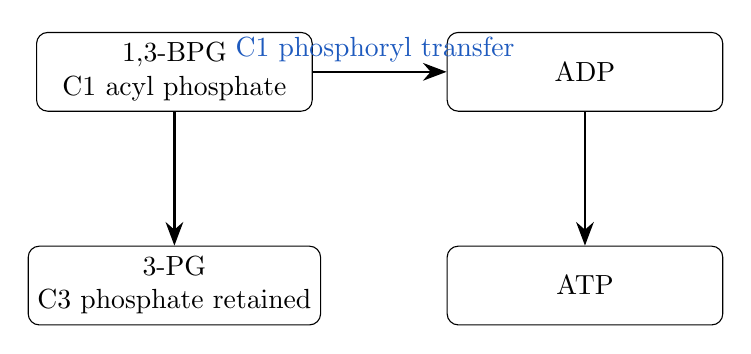
\begin{tikzpicture}[
  box/.style={
    draw,rounded corners,align=center,
    minimum width=3.5cm,minimum height=1cm
  },
  arr/.style={-{Stealth[length=3mm]},thick},
  node distance=17mm
]

\node[box] (bpg) {1,3-BPG\\C1 acyl phosphate};
\node[box,right=of bpg] (adp) {ADP};
\node[box,below=of adp] (atp) {ATP};
\node[box,below=of bpg] (pg) {3-PG\\C3 phosphate retained};

\draw[arr] (bpg) -- node[above,align=center] {
  \textcolor{phos}{C1 phosphoryl transfer}
} (adp);

\draw[arr] (adp) -- (atp);
\draw[arr] (bpg) -- (pg);

\end{tikzpicture}
\end{center}

\textbf{Chemical changes}

\begin{enumerate}
  \item The high-energy C1 acyl phosphate is transferred to ADP.
  \item ATP is formed.
  \item The C3 phosphate remains attached to the carbon skeleton.
  \item The product is 3-phosphoglycerate.
\end{enumerate}

\textbf{Reaction classification:} Substrate-level phosphorylation.
There is no net oxidation-reduction reaction.

\[
\boxed{\text{ATP produced: 2 per glucose}}
\]

% =========================================================

\subsection*{STEP 8. 3-phosphoglycerate $\rightarrow$ 2-phosphoglycerate}

\textcolor{enz}{\textbf{Enzyme: Phosphoglycerate mutase}}

\[
\ce{3-PG <=> 2-PG}
\]

\begin{center}
\resizebox{0.96\linewidth}{!}{$
\begin{aligned}
\text{\textbf{3-phosphoglycerate:}}\quad
&\PGthree
\\[5pt]
&\xrightleftharpoons{\text{Phosphoglycerate mutase}}
\\[5pt]
\text{\textbf{2-phosphoglycerate:}}\quad
&\PGtwo
\end{aligned}
$}
\end{center}

\textbf{Chemical changes}

\begin{enumerate}
  \item The phosphate is relocated from C3 to C2.
  \item The enzyme can use a transient bisphosphorylated intermediate.
  \item The final product contains the phosphate on C2.
\end{enumerate}

\[
\boxed{
\mathrm{C3{-}OPO_3 \longrightarrow C2{-}OPO_3}
}
\]

The phosphate is rearranged, not added from ATP.

\textbf{ATP consumed or produced: 0.}

% =========================================================

\subsection*{STEP 9. Dehydration of 2-phosphoglycerate}

\textcolor{enz}{\textbf{Enzyme: Enolase}}

\[
\ce{2-PG <=> PEP + H2O}
\]

\begin{center}
\resizebox{0.96\linewidth}{!}{$
\begin{aligned}
\text{\textbf{2-phosphoglycerate:}}\quad
&\PGtwo
\\[5pt]
&\xrightleftharpoons{\text{Enolase}}
\\[5pt]
\text{\textbf{Phosphoenolpyruvate:}}\quad
&\PEP
\end{aligned}
$}
\end{center}

\textbf{Chemical changes}

\begin{enumerate}
  \item Water is eliminated from the substrate.
  \item The carbon skeleton develops a carbon-carbon double bond.
  \item The phosphate remains attached to the enol oxygen.
  \item PEP is produced.
\end{enumerate}

\[
\boxed{\ce{2-PG -> PEP + H2O}}
\]

\textbf{Electron movement:} Bond electrons are redistributed
during the elimination reaction to create the double bond.

\textbf{ATP produced: 0.}

% =========================================================

\subsection*{STEP 10. Phosphate transfer from PEP to ADP}

\textcolor{enz}{\textbf{Enzyme: Pyruvate kinase}}

\[
\ce{
PEP + ADP + H+
-> Pyruvate + ATP
}
\]

\begin{center}
\resizebox{0.96\linewidth}{!}{$
\begin{aligned}
\text{\textbf{PEP:}}\quad
&\PEP
\\[5pt]
&\xrightarrow[\text{Mg}^{2+},\ \text{K}^{+}]
{\text{Pyruvate kinase;\ ADP}\rightarrow\text{ATP}}
\\[5pt]
\text{\textbf{Pyruvate:}}\quad
&\Pyruvate
\end{aligned}
$}
\end{center}

\textbf{Chemical changes}

\begin{enumerate}
  \item The phosphate group of PEP is transferred to ADP.
  \item ATP is produced.
  \item The three-carbon skeleton forms the enol form of pyruvate.
  \item Keto-enol tautomerization yields the more stable keto form
  of pyruvate.
\end{enumerate}

\textcolor{phos}{\textbf{Transfer:}}
\[
\ce{PEP + ADP -> Pyruvate + ATP}
\]

The favorable tautomerization of the pyruvate product contributes
to the thermodynamic favorability of this reaction.

\[
\boxed{\text{ATP produced: 2 per glucose}}
\]

% =========================================================
\newpage
\section*{COMPLETE PATHWAY ACCOUNTING}
% =========================================================

\subsection*{All ten reactions}

\small

\begin{tabular}{c p{5.1cm} p{8.0cm} c}
\toprule
\textbf{Step} & \textbf{Enzyme} & \textbf{Reaction} &
\textbf{ATP per glucose}\\
\midrule
1 & Hexokinase &
Glucose $\rightarrow$ glucose-6-phosphate & $-1$\\

2 & Phosphoglucose isomerase &
Glucose-6-phosphate $\rightarrow$ fructose-6-phosphate & 0\\

3 & Phosphofructokinase-1 &
Fructose-6-phosphate $\rightarrow$ fructose-1,6-bisphosphate & $-1$\\

4 & Aldolase &
Fructose-1,6-bisphosphate $\rightarrow$ GAP + DHAP & 0\\

5 & Triose phosphate isomerase &
DHAP $\rightarrow$ GAP & 0\\

6 & GAP dehydrogenase &
GAP $\rightarrow$ 1,3-BPG; NAD$^+$ $\rightarrow$ NADH & 0\\

7 & Phosphoglycerate kinase &
1,3-BPG $\rightarrow$ 3-PG; ADP $\rightarrow$ ATP & $+2$\\

8 & Phosphoglycerate mutase &
3-PG $\rightarrow$ 2-PG & 0\\

9 & Enolase &
2-PG $\rightarrow$ PEP + water & 0\\

10 & Pyruvate kinase &
PEP $\rightarrow$ pyruvate; ADP $\rightarrow$ ATP & $+2$\\

\bottomrule
\end{tabular}

\normalsize

\subsection*{Net reaction}

\[
\boxed{
\begin{aligned}
\ce{Glucose}
&+\ce{2 NAD+}
+\ce{2 ADP}
+\ce{2 P_i}
\\
&\longrightarrow
\ce{2 Pyruvate}
+\ce{2 NADH}
+\ce{2 H+}
+\ce{2 ATP}
+\ce{2 H2O}
\end{aligned}
}
\]

The displayed net reaction uses a common biochemical protonation
convention.

\subsection*{Final balance}

\begin{center}
\begin{tabular}{lr}
\toprule
\textbf{Quantity} & \textbf{Net result}\\
\midrule
Glucose consumed & 1\\
Pyruvate produced & 2\\
ATP consumed & 2\\
ATP produced & 4\\
Net ATP & 2\\
NADH produced & 2\\
Carbon dioxide released & 0\\
FAD consumed & 0\\
\bottomrule
\end{tabular}
\end{center}

\subsection*{Key distinctions}

\begin{enumerate}
  \item Steps 1 and 3 consume ATP to phosphorylate sugars.
  \item Step 6 oxidizes GAP and reduces NAD$^+$.
  \item Step 6 incorporates inorganic phosphate into 1,3-BPG.
  \item Step 7 transfers the C1 phosphate of 1,3-BPG to ADP.
  \item Step 8 moves the phosphate from C3 to C2.
  \item Step 9 removes water and forms PEP.
  \item Step 10 transfers the phosphate of PEP to ADP.
  \item Steps 7 and 10 are the ATP-generating reactions.
\end{enumerate}

\end{document}
